\documentclass[
	letterpaper, % Paper size, specify a4paper (A4) or letterpaper (US letter)
	10pt, % Default font size, specify 10pt, 11pt or 12pt
]{class}

\usepackage{caption}
\usepackage{soul}
\usepackage{subcaption}

\addbibresource{bibliography.bib} % Bibliography file (located in the same folder as the template)

%----------------------------------------------------------------------------------------
%	REPORT INFORMATION
%----------------------------------------------------------------------------------------

\title{GPU Computing\\Parallel implementation of Dijkstra's Algorithm} % Report title

\author{Tricella Davide 08361A} % Author name(s), add additional authors like: '\& James \textsc{Smith}'

\date{\today} % Date of the report

%----------------------------------------------------------------------------------------

\begin{document}

\maketitle % Insert the title, author and date using the information specified above

\begin{center}
    \begin{tabular}{l r}
        Instructor: Professor \textsc{Grossi Giuliano}
    \end{tabular}
\end{center}

%----------------------------------------------------------------------------------------
%	ABSTRACT
%----------------------------------------------------------------------------------------

\begin{abstract}
    The purpose of this paper is to describe the implementation and benchmarking of various parallel implementations of Dijkstra's Algorithm to solve the shortest path problem.
\end{abstract}

%----------------------------------------------------------------------------------------
%	TOC
%----------------------------------------------------------------------------------------

\tableofcontents

%----------------------------------------------------------------------------------------
%	INTRODUCTION
%----------------------------------------------------------------------------------------

\section{Introduction}

The problem of shortest path in a graph consists in finding the path, from node A to node B,
which minimizes the sum of edges weights of which the path is composed.\\

\begin{center}
    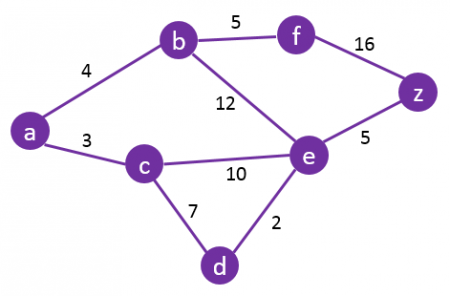
\includegraphics[width=10cm]{../images/graph.png}
    \captionof{figure}{Graph with edge weights}
\end{center}

In particular, the algorithm used for this document aim to solve the all-pairs shortest path problem,
which consists of finding the lenght of the shortest path for all the pairs of nodes.\\

The algorithm assumes that there are not negative weights and that the graph is undirected without isolated parts.\\

This problem is tackled in a lot of practical applications, like road networks path-finding, telecommunication routing and robot navigation.

\printbibliography % Output the bibliography

%----------------------------------------------------------------------------------------

\end{document}